%
%このファイルは日本バーチャルリアリティ学会論文集用スタイルファイル
%jvrst2e.sty(ver.2.0) を利用したサンプルファイルです。
%
\documentclass[a4paper,twoside]{jarticle}
\usepackage{tvrsj2e}
\usepackage[dvipdfmx]{graphicx}

%和文タイトル 論文のヘッダ部分にも出力されます。  
\jtitle{
    日本VR学会論文誌論文執筆ガイドライン}

%著者日本名   
\jauthor{
    人工 太郎\thanks{バーチャル大学} \hspace{10mm}
    現実 花子\thanks{リアリティ研究所}}

%英文タイトル
\etitle{
    Guidelines for Writing Papers for VRSJ Transaction}

%著者英文名
\eauthor{
    Taro Jinko\thanks{Virtual University} and
    Hanako Genjitsu\thanks{Reality Research Institute}}

%西暦(4桁まで)
\YEAR{2007}
\VOL{1}	
\NO{1}

%論文の種別に合わせる
\TYPE{基礎論文}
%\TYPE{応用論文}
%\TYPE{コンテンツ論文}
%\TYPE{総説論文}
%\TYPE{ショートペーパー}

%論文のヘッダにつける著者名
\AUTHOR{人工・現実}

\begin{document}

%maketitle は abstract と keyword の後に入れてください。

\begin{abstract}
This paper describes guidelines for writing papers for VRSJ
Transaction. Detailed instructions on font size and styles of all
elements in the paper, including headers and footnotes, paper title
and authors, section and subsection headings, and reference list. Some
specific notes for respectively review and final papers are also
stated. All papers submitted for VRSJ Transaction are expected to
follow these guidelines: it is very important for the aesthetic
consistency of papers through a volume that each author strictly
follows the guidelines. This document also serves as a sample document
that provides authors a concrete appearance of formatted pages.
\end{abstract}

\begin{keyword}	
format and style, guideline, VRSJ transaction, virtual reality
\end{keyword}

\maketitle	

\section{はじめに}

本稿では日本VR学会論文誌に投稿する際の論文のスタイルおよび書式について
説明する。この論文誌が対象とする分野・領域、論文のカテゴリなどについて
は投稿規程\cite{toukou}を、投稿の手続きについては投稿の手引き
\cite{tebiki}を参照していただきたい。なお、査読の方法・手順については
論文委員会規程\cite{iinkai}に記述されている。査読はシングルブラインド
(著者の情報が査読者に見える状態)で行われる。したがって、査読用の原稿
においても著者の氏名や所属、著者自身らによる関連研究の参考文献などが漏
れなく記述されている必要がある。

以下、2章では論文の構成と記述の形式およびスタイルについて、3章では図表
などの要素の作成の注意について述べる。これらは論文誌として誌面の統一感
を得るための重要な事項であり遵守していただきたい。カメラレディ原稿(印
刷用原稿)では印刷結果の再現性や品質の観点から原稿作成の過程で配慮が必
要であり、これらにかかる注意点について4章で述べる。

\section{ページの構成}

\subsection{用紙と余白}
用紙はA4サイズとし、左右の余白はそれぞれ20mm、上下の余白は20mmおよび
24mmとする。したがって、テキスト領域は幅170mm高さ253mmとなる。タイトル
ページ(1ページ目)の左上の余白には論文カテゴリ名(付録A.1参照)(明朝体14
ポイント・下線)を記述する。ショートペーパーの場合には、サブカテゴリを
基礎・応用・コンテンツの中から選択し、「ショートペーパー(基礎)」のよう
に括弧付きで表示する。次ページ以降は、偶数ページには上の余白中央に誌名
(ゴシック体7ポイント)、巻号・発行年(Times-Roman Bold 7ポイント)を「日
本バーチャルリアリティ学会論文誌 Vol.12, No.1, 2007」の形式で、奇数ペー
ジには同じく上の余白中央に和文著者姓および和文論文題目(ゴシック体7ポイ
ント)を「佐藤・鈴木: ○○○に関する研究」の形式で記述する。なお、著者
が3名以上の場合は筆頭著者のみを挙げて「佐藤他」などとして良い。また、
和文論文題目が長く1行に収まらない場合には簡略化した題目を記述する。

\subsection{論文タイトル}
タイトルページには、テキスト領域には本文に先立ち、
①和文論文題目(ゴシック体17ポイント)、
②和文著者氏名(明朝体14ポイント)、
③英文論文題目(Times-Roman Bold 10ポイント)、
④英文著者氏名(Times-Roman 10ポイント)、
⑤英文アブストラクト(Times-Roman Bold 10ポイント)、
⑥英文キーワード(Times-Roman Bold 10ポイント)を
記述する。英文アブストラクトは100語程度、英文キーワードは5個程度とする。
これらはページの左右中央に幅145mmの領域
に収まるように配置する。また、項目の間には適当なスペースを挿入する。一
方、ページの左下に脚注として、
⑦和文著者所属(明朝体7ポイント)および
⑧英文著者所属(Times-Roman 7ポイント)を記述し、
和文著者氏名および英文著者氏名に脚注記号をつけて参照する。

\subsection{本文}
上述の論文題目から英文キーワードの記述のあと適当なスペースを空けて本文
およびを記述する。本文はテキスト領域に2段組で記述する。段の間隔は10mm
とする。したがって、1つの段の幅は80mmとなる。本文は必要に応じて章およ
び節に区切って記述する。なお、各論文を章とみなし、論文の中の区切りを節
とする流儀もあり、それに従っても構わない。その場合は以下の説明で章を節、
節を小節と読み替えていただきたい。章の見出しは章番号および章題目(ゴシッ
ク体10ポイント・中央配置)を「2 背景と目的」の形式で記述する。また、こ
の前後には適当なスペースを挿入する。一方、節の見出しは章節番号および節
題目(ゴシック体10ポイント・左揃え)を「2.1 従来の研究」の形式で記述する。
項番号および項題目などさらに細かい区切りの形式については著者の判断で決
めてよい。タイトルに続いて文章段落(明朝体10ポイント・インデント)を開始
する。段落頭のインデントは1文字程度とする。句読点は「、。」または「,.」
のいずれかに統一する。

\subsection{謝辞}
必要に応じて、本文の後に謝辞を記述することができる。謝辞の見
出しは章題目と同様のスタイル(ゴシック体10ポイント・中央配置)で「謝辞」
と記述する。ただし、章番号はつけない。文章段落は本文と同じスタイルとす
る。

所属機関等の倫理委員会の承認を得て実施された研究については、その旨を明
記する。また、競争的資金等により実施された研究で謝辞の記述を求められて
いる場合も、ここに記述する。

\subsection{参考文献リスト}
本文に続いて参考文献のリストを記述する。参考文献リストの見出しは章題目
と同様のスタイル(ゴシック体10ポイント・中央配置)で「参考文献」と記述す
る。ただし、章番号はつけない。文献の各項目は先頭に参照番号(Times-Roman
10ポイント)、を角括弧をつけて表示する。それに続く個々の文献情報(明朝体
9ポイントまたはTimes-Roman 9ポイント)は参照に必要十分な内容を記述す
る(たとえば、論文誌や予稿集は\cite{bib1,bib2,bib3,bib4}、著書であれば
\cite{bib5,bib6})。姓名の記法や誌名巻号の略記法など形式について厳密な
指定はしないが、リストの中では統一がとれていることが望ましい。

\subsection{付録}
必要に応じて、謝辞の後に付録を記述することができる。付録の見出しは本文
の章節と同様の形式とするが、見出しは「A 付録」とする。

\subsection{受付日}
受付年月日(Times-Roman Boldおよびゴシック体 10ポイント)を「(2007年3月
27日受付)」の形式で記述する。なお、査読原稿の段階では有効な日付を記入
する必要はない。

\subsection{著者紹介}
著者紹介の見出しは(明朝体10ポイント・中央配置)で「[著者紹介]」とする。
個々の著者について、左寄せで著者氏名(ゴシック体10ポイント)および会員・
学生会員・非会員の別(明朝体10ポイント)を記述し、その下に左寄せで顔写真
(幅15mm高さ20mm)、その右に略歴(明朝体9ポイント)を記述する。なお、ショー
トペーパーにおいては、著者紹介を省略してもよい。

\section{図表と参照}

\subsection{図表}
図表は対象とするものやことを分かり易く説明するための手段であり、積極的
に活用したい。図表を使用するかどうかの判断は、同様の内容を文章で説明し
た場合と比較して誌面を節約できるかどうかということが一つの目安である。

図は線画・写真とも十分に鮮明なものを用い、図中の文字は本文の文字サイズ
と釣り合う大きさとする。和文表題(ゴシック体 9ポイント)と英文表題
(Times-Roman 9ポイント)を図の下につける。 和文表題の形式は「図1 シス
テム構成」、英文表題の形式は「Fig.1 Configuration of system」とする
(図\ref{fig:zu}参照)。
必要に応じて2つの段を通した図を用いてよい。

\begin{figure}[ht]
\begin{center}
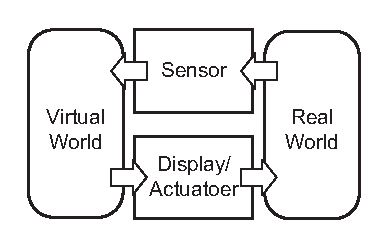
\includegraphics[scale=1.0]{zu.eps}
\end{center}
\caption{システム構成}
\ecaption{Configuration of system}
\label{fig:zu}
\end{figure}

表についても、文字は本文の文字サイズと釣り合う大きさとする。
和文表題(ゴシック体 9ポイント)と英文表題
(Times-Roman 9ポイント)を表の上につける。 和文表題の形式は「表1 精度
と時間」、英文表題の形式は「Table.1 Accuracy and time」とする
(表\ref{tab:ta}参照)。
表についても必要に応じて2つの段を通したものを用いてよい。

\begin{table}[ht]
\caption{精度と時間}
\ecaption{Accuracy and time}
\label{tab:ta}
\begin{center}
\begin{tabular}{|c|c|c|}
\hline
subject & accuracy [mm] & time [ms]\\ \hline
s1      & 23       & 538  \\ \hline
s2      & 36       & 375  \\ \hline
s3      & 21       & 412  \\ \hline
s4      & 15       & 736  \\ \hline
\end{tabular}
\end{center}
\end{table}

\subsection{参照}
参考文献および図表は本文中で必ず参照されなければならない。参考文献は参
照番号を用いて「\cite{bib1}」の形式で参照する。同様に図表はそれぞれ
「図\ref{fig:zu}」「表\ref{tab:ta}」の形式で参照する。

\section{カメラレディ原稿作成の注意}

紙媒体の論文誌ではモノクロ印刷となるので、その場合でも視認性に問題がな
いことを確認すること。とくに写真のコントラストやグラフの線の区別などが
読者に混乱を与えないように配慮する。極端に細い線は印刷されない場合があ
る。電子原稿(PDF)の作成では図表の解像度が600dpi以上となるように、また、
フォントはすべて埋め込む設定を使用する。

\section*{謝辞}
日本VR学会の会員各位および論文誌への投稿者各位に感謝する。
本研究は○○研究費(課題番号○○○○)の助成を受けたものである。なお、
本研究は○○大学○○学部倫理委員会の承認(承認番号○○○○)をうけて、実
施されたものである。

\begin{thebibliography}{99}
\bibitem{toukou}
日本VR学会論文投稿規程:\\
http://www.vrsj.org/monograph/rule.html\#kitei
\bibitem{tebiki}
日本VR学会論文投稿の手引き:\\
http://www.vrsj.org/monograph/manual.html
\bibitem{iinkai}
日本VR学会論文委員会規程:\\
http://www.vrsj.org/about/rule2.html\#ronbun
\bibitem{bib1}
著者1, 著者2: バーチャルリアリティに関する研究; ○○論文誌, 巻(号), 
始頁-終頁 (発行年.月)
\bibitem{bib2}
Author1, Author2: A study on Virtual Reality; Journal Name, vol(no), 
page-page (year.month)
\bibitem{bib3}
著者1, 著者2: バーチャルリアリティ環境の評価; ○○学会大会, 始頁-終頁 
(発行年.月)
\bibitem{bib4}
Author1, Author2: Evaluation of Virtual Reality Environment;
Conference Name, page-page (year.month)
\bibitem{bib5}
著者1, 著者2, 編者(編): バーチャルリアリティの本; ○○出版, 所在地 (発行年.月)
\bibitem{bib6}
Author1, Author2, Editor(Ed.): A book of Virtual Reality; Publisher, Address (year.month)
\end{thebibliography}

\section*{A 付録}
\subsection*{A.1 投稿カテゴリ}
本論文誌の投稿カテゴリは次の5つのいずれかとする。以下、投稿規程
\cite{toukou}より抜粋。

\noindent
{\bf 基礎論文}

標準6ページ、原則10ページまで。バーチャルリアリティに
関する理論、システム設計、評価手法、人間科学等の知見に関する新たな提案。 

\noindent
{\bf 応用論文}

標準6ページ、原則10ページまで。バーチャルリアリティの
応用(産業応用、医療応用等)に重点をおきながら、新しい概念や技術を提案
するもの。

\noindent
{\bf コンテンツ論文}

標準6ページ、原則10ページまで。バーチャルリアリ
ティをメディアとして用いた表現内容に関する新しい提案(アート、エンタテ
イメント、ビジネス等)。

\noindent
{\bf 総説論文}

標準6ページ、原則10ページまで。新たな観点のもとにバー
チャルリアリティに関する知見を整理したもの(レビューペーパー、チュート
リアルペーパー等)。

\noindent
{\bf ショートペーパー}

標準2ページ、4ページまで。バーチャルリアリティにおける基礎、応用、コン
テンツに関する速報的な論文。

%採択受付日を記入してください。投稿時および日付がわからない場合にはコ
%メントアウトしておいてください。
\saitaku{2009年5月14日}

%著者紹介
\begin{biography}
%\profile{名前}{m:正会員、s:学生会員、空白:非会員}{顔写真のepsファイル名}{略歴}
%顔写真のepsファイルは解像度の高いもので、サイズが縦2.2cm、横1.7cm程度
%になるようにしてください。うまく貼れない場合は空欄にしておいて、後ほ
%どペーストしてください。
\profile{人工 太郎}{m}{kao.eps}{
19XX年○○大学大学院○○研究科修了。
19XX年バーチャル大学○○学科助手、20XX年 同学科講師、現在に至る。
人工現実感および感覚情報提示に関する研究に従事。博士(○○)。}

\profile{現実 花子}{m}{kao.eps}{
19XX年○○大学大学院○○研究科修了、同年リアリティ研究所研究員、現在に
至る。認知心理および感覚受容に関する研究に従事。博士(○○)。}
\end{biography}
\end{document}
